\documentclass[11pt, a4paper, tikz]{article}

\usepackage[english]{babel} %language
\usepackage[utf8]{inputenc} %UTF-8 encoding
\usepackage[margin=0.5in]{geometry} %smaller margin
\usepackage{amssymb} %\nexists \mathbb
\usepackage{amsmath}
\usepackage{amsthm}
\usepackage{graphicx}
\usepackage{polynom}
\usepackage{mathtools}
\usepackage{enumitem}

\usepackage{xlop}
\usepackage[dvipsnames]{xcolor}
\usepackage{tcolorbox}

\definecolor{formulationFrameColor}{RGB}{150,160,190}
\definecolor{formulationBackgroundColor}{RGB}{240,245,250}

\newtcolorbox{formulationBox}{
	colframe=formulationFrameColor,
	colback=formulationBackgroundColor
}

\usepackage{tikz}   
\usepackage{pgfplots}

\pgfplotsset{compat=1.6}

\pgfplotsset{soldot/.style={color=red,only marks,mark=*}} \pgfplotsset{holdot/.style={color=red,fill=white,only marks,mark=*}}

\pgfplotsset{compat=newest} % used to declare my style command.  

\newcommand{\newpara}{
	\vskip 2mm
}

\newcommand{\centsection}[1]{
	\section*{\centering{#1}}
}

\newcommand{\centsubsection}[1]{
	\subsection*{\centering{#1}}
}

\newcommand{\myOver}[2]{
	\ensuremath{\overset{\kern2pt #1}{#2}}
}

\newcommand{\final}[1]{
	$\mathcal{F}($#1$)$
}

\renewcommand{\qed}{\hfill\blacksquare}

\newcommand{\Lim}[1]{\raisebox{0.5ex}{\scalebox{0.8}{$\displaystyle \lim_{#1}\;$}}}
\newcommand{\Inf}[1]{\raisebox{0.5ex}{\scalebox{0.8}{$\displaystyle \inf_{#1}\;$}}}
\newcommand{\Sup}[1]{\raisebox{0.5ex}{\scalebox{0.8}{$\displaystyle \sup_{#1}\;$}}}
\newcommand{\Sum}[2]{\displaystyle \sum_{#1}^{#2}}
\newcommand{\Int}[2]{\displaystyle \int_{#1}^{#2}}

\newcommand{\naturals}{
	\ensuremath{\mathbb{N}}
}
\newcommand{\integers}{
	\ensuremath{\mathbb{Z}}
}
\newcommand{\rationals}{
	\ensuremath{\mathbb{Q}}
}
\newcommand{\reals}{
	\ensuremath{\mathbb{R}}
}
\newcommand{\complexes}{
	\ensuremath{\mathbb{C}}
}

\graphicspath{ {./media/} }

\begin{document}
	\title{\textbf{Chapter 2 — Section A}}
	\maketitle
	%\setcounter{section}{3}
	\centsection{Exercise 1}
	
	\begin{formulationBox}
		Prove that if $A$ and $B$ are subsets of $\reals$ and $|B|=0$, then $|A\cup B| = |A|$.
	\end{formulationBox}
	
	By theorem 2.5, \textit{outer measure preserves order}, as $A$ and $A\cup B$ are subsets of $\reals$ with $A\subseteq A\cup B$, then $|A| \leq |A\cup B|$.
	\newpara
	Now, by theorem 2.8, \textit{countable subadditivity of outer measure}, and as it trivially implies finite subadditivity, we have $|A\cup B| \leq |A| + |B| = |A| + 0 = |A|$.
	\newpara
	As we have both $|A\cup B| \leq |A|$ and $|A| \leq |A\cup B|$, we get $|A\cup B| = |A|$.
	
	$\qed$
	
	\centsection{Exercise 14}
	
	\begin{formulationBox}
		Consider the following figure, which is drawn accurately to scale.
		
		\centering{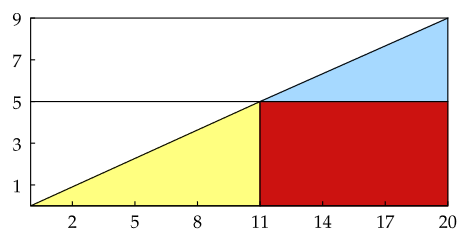
\includegraphics[scale=0.7]{./2A-14-1}}
		
		\begin{enumerate}[label=\alph*)]
			\item Show that the right triangle whose vertices are $(0,0)$, $(20, 0)$ and $(20, 9)$ has area $90$.
			\item Show that the yellow (lower) right triangle has area $27.5$.
			\item Show that the red rectangle has area $45$.
			\item Show that the blue (upper) right triangle has area $18$.
			\item Add the results of parts b), c) and d), showing that the area of the colored region is $90.5$.
			\item Explain why the results obtained in a) and e) differ.
		\end{enumerate}
	\end{formulationBox}

	\begin{enumerate}[label=\alph*)]
		\item Such triangle has height $9-0=9$ and width $20-0=20$, so its area is $\frac{20\cdot9}{2} = 90$.
		\item Similarly, the area of the yellow triangle is $\frac{(11-0)(5-0)}{2} = 27.5$.
		\item The area of the red rectangle is $(20-11)(5-0) = 45$.
		\item The area of the blue triangle has area $\frac{(20-11)(9-5)}{2} = 18$.
		\item The area of the colored region is $27.5 + 45 + 18 = 90.5$.
		\item The colored region is actually not a triangle, just a right trapezoid with an angle very close to $180^\circ$. The triangle described in part a) has a slope of $\frac{9}{20}$, while the yellow and blue triangles have slopes $\frac{5}{11}$ and $\frac{4}{9}$ respectively. The following picture illustrates that there is indeed a separation between the lines, although it is hard to see without zooming in.
		
		\centering{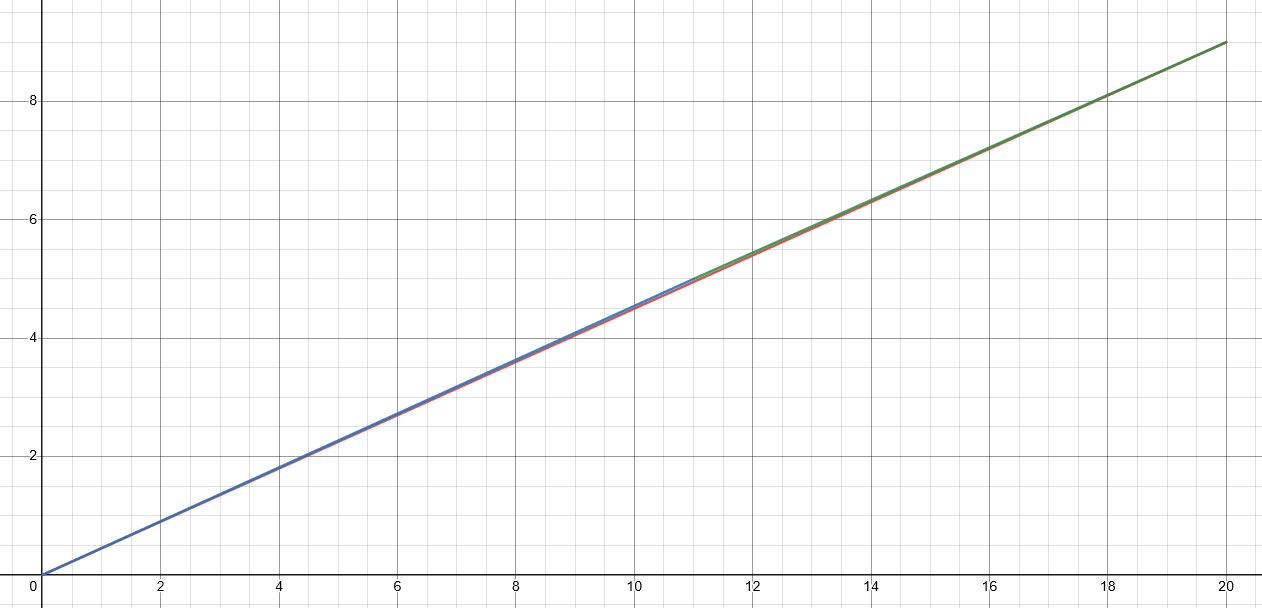
\includegraphics[scale=0.4]{./2A-14-2}}
	\end{enumerate}
	
	I kind of feel like this exercise was a bit off-topic, as in it has nothing to do with the new concepts learned in this chapter.
\end{document}